\subsection{Добавяне на библиотеки}
За да добавим библиотека в Rust трябва да я добавим в Cargo.toml файла под
секцията наречена dependencies. Синтакса за добавяне е много прост, а именно в
ляво името на библиотеката, посредата знака за равно и вдясно версията на
библиотеката.
\begin{figure}[!htb]
  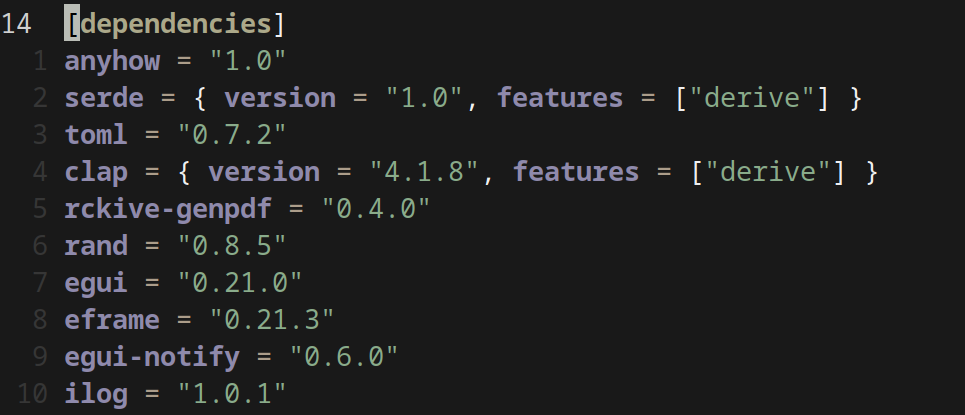
\includegraphics[scale=0.7]{rust-deps.png}
  \centering
  \caption{Ситаксис за добавяне на библиотеки}
  \label{fig:rust-deps}
\end{figure}

\subsubsection{Конзолни аргументи}
Аргументите на конзолата са параметри, предавани на програмата преди изпълнение
и в командния ред. В Rust аргументите могат да бъдат достъпени чрез
функцията \textit{std::env::args()}, която връща итератор над аргументите като списък от
низове.

За да вземем подходящата информация за приложението, може да напишeм наш собствен
анализатор или да изплозваме една от многото различни библиотеки за работа с
конзолни аргументи. Една от най-често използваните библиотеки е clap (Console Line
Argument Parser).

Clap ни предоставя с \textit{clap::Parser} макрото, което при компилирането на програмата
анализира структурата от данни и автоматично търси командните аргументи при
изпълнение на програмата. Също тъка, проверява кои аргументи са маркирани като
задължителни или такива със стойност по подразбиране. [Фигура \ref{fig:clap-example}]
\begin{figure}[!htb]
  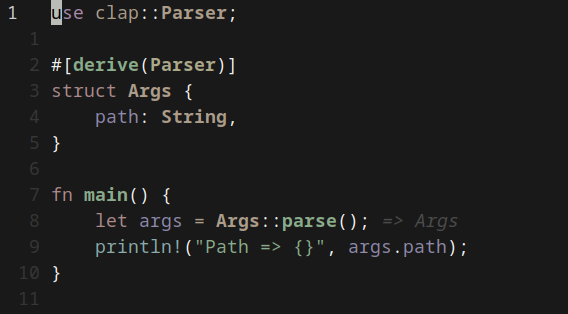
\includegraphics[scale=0.7]{clap-example}
  \centering
  \caption{Четене на командни аргументи с \textit{clap}}
  \label{fig:clap-example}
\end{figure}

При въвеждане на грешни аргументи или при липсата на задължителните такива, \textit{clap}
показва автоматично генерираното помощно съобщение на потребителя.
\begin{figure}[!htb]
  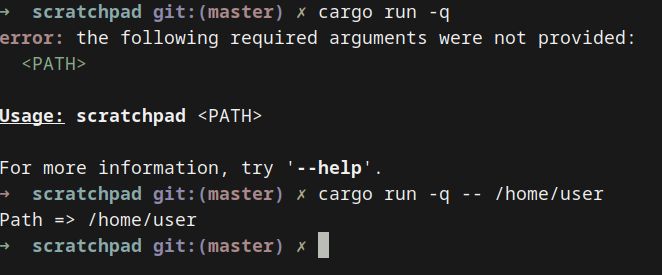
\includegraphics[scale=0.7]{clap-help}
  \centering
  \caption{Генерираното помощно съобщение от \textit{clap}}
  \label{fig:clap-help}
\end{figure}

\subsubsection{Serde}
\textit{Serde} е framework за ефективно сериализиране и десериализиране на структури от данни в Rust.

Екосистемата на \textit{Serde} се състои от структури от данни, които знаят как да
сериализират и десериализират себе си заедно с формата на данните. \textit{Serde} предоставя слой, чрез
който тези две групи взаимодействат помежду си, позволявайки всяка поддържана
структура от данни да бъде сериализирана и десериализирана с помощта на всеки
поддържан формат на данни.

Докато много други езици разчитат на runtime среда (като Dotnet) за
сериализиране на данни, \textit{Serde} вместо това е изградена върху много добрата
интерфес система на Rust.

Структура от данни, която знае как да сериализира и десериализира сама себе си,
е тази, която използва интерфейсите на \textit{Serde} за сериализиране и десериализиране
(или използва атрибута derive на \textit{Serde} за автоматично генериране на интерфеси
по време на компилация). По този начин се избягват забавянето от употребата на
runtime среда.

Всъщност в много ситуации взаимодействието между структурата на данните и
формата на данните може да бъде напълно оптимизирано от Rust компилатора,
оставяйки сериализацията на \textit{Serde} да се изпълни със същата скорост като
ръчно написан сериализатор в езици от по-ниско ниво като \textit{C}.

\subsubsection{Toml}
Toml (Tom's Obvious Minimal Language) е файлов формат за съхранение на
софтуерни конфигурации. Този формат ще бъде използван за съхраняване на
настройките, въпросите и друга информация за тестовете. За да добавим подръжка
за този формат в Rust, трябва да инсталираме Toml библиотека, която използва
Serde за преобразуването на файл в обект и обратно.

% TODO: explain how toml is integrated with serde
% TODO: exmaple?

\subsubsection{genpdf}
genpdf е библиотека за генериране на PDF документи на високо ниво, изградена от
две по-малки библиотеки от по-ниско ниво. Тя се грижи за оформлението на
страницата, подравняването на текста и изобразява дървовидната структура на
документа в PDF файла.
